\Chapter{Review of the literature}{Part I: Microelectronics design}
\label{cha:rol.icdesign}

\begin{summary}
\lipsum[1]
\end{summary}

\section{Introduction}

\section{2D architecture and its limitations}

In order to continuously improve the performance of integrated circuits (IC), technologists deploy enormous efforts to produce IC manufacturing process that is compelling to follow the well-known Moore's Law (see Fig. \ref{fig:mooreslaw}). This empirical law predicts a doubling of the transistors' integration each 18 months and therefore increasing logic capacity of the circuit per unit area. 

\begin{figure}
\begin{center}
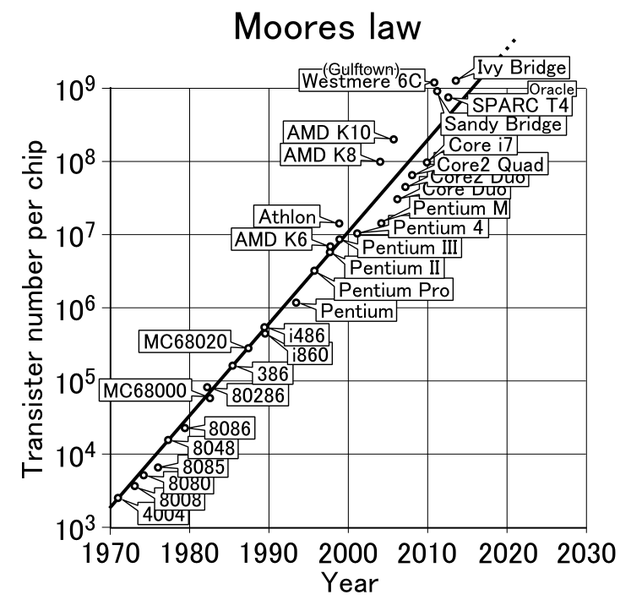
\includegraphics[width=0.75\linewidth]{mooreslaw.png}
\end{center}
\vspace{-0.5cm}
\caption{Moore's law \cite{mooreslawpic}}
\label{fig:mooreslaw}
\end{figure}

The improvements of 2D architectures are primarily driven by the reduction of the transistor size. By reducing transistor dimensions, the switching speed is increased thanks to the shorter distance between the source and the drain, implying an improvement of the overall speed of the designs.

However, as the transistor size is decreasing, the observed improvement is also getting smaller. Indeed, a smaller transistor allows higher device density but will slightly increase the total delay (sum of gate and interconnection delays). Also, power consumption is increased due to higher leakage and increasing interconnection wire length \cite{5227192}.

With the miniaturization, quantum effects such as quantum tunnelling will significantly affect how a transistor behave \cite{1240081}.

In addition to these physical aspects, economical considerations that will hinder the IC evolution beyond 20nm have to be taken into account \cite{5227192,PFF10}.

In order to overcome these limitations, new technologies have been proposed such as the carbon nanotubes \cite{tans1998room}, the nanowire transistors \cite{doi:10.1021/nl025875l}, the single-electron transistors \cite{citeulike:4194929}, but also the 3D-Stacked Integrated Circuits (3D-SIC) proposed by the academic and industrial communities. The latter has been often cited as the most prominent one~\cite{659500}.

\section{3D integration}

Most of the current ICs are designed with electronic components (i.e. transistors) that are planar (although multi-gate transistors, such as finFETs tends to extend in the 3rd dimension) interconnected using up to a maximum of 12 (also planar) wiring (metal) layers per circuit. Those conventional ICs can thus be considered to be two-dimensional (2D)-ICs since the interconnections are predominantly made in a planar fashion~\cite{1393404,fujitsu08}. As a major evolution of 2D-ICs, 3D-SICs are designed with multiple traditional 2D-ICs (that are manufactured independently, using standard CMOS technology) that are assembled (stacked) vertically in 3D-tiers. Different 2D circuits communicate between tiers using vertical interconnections that need to connect front side of the chip and the backside, i.e. they need to traverse bulk silicon. These connections, known as \--- Through Silicon Vias (TSV), can be today manufactured with satisfactory geometrical properties, namely their diameter, pitch and height, allowing efficient integration of real-world systems~\cite{1705326,5746413}. This is shown in Fig.~\ref{fig:3D_SIC_SOC2010}, where 2 dies, oriented face down are connected. An active component (i.e. logic gate) of the T1 is connected to the T2 using a TSV, back side metallization layer (to enable TSV placement anywhere in the T1 die), and micro-bump on the top layer of the T2, that is then connected, through a series of metal layers of the T2, to the active component of the top tier (T2).

\begin{figure}[h!]
\begin{center}
%\includegraphics[width=1\linewidth]{3D_SIC_SOC2010.png}
\includegraphics[width=0.75\linewidth]{3DSIC.pdf}
\end{center}
\vspace{-0.5cm}
\caption{Illustration of the wiring properties of a 3D-SIC}
\label{fig:3D_SIC_SOC2010}
\end{figure}

The benefits of using 3D-ICs are numerous and have been already pointed out in the literature very often over the past few years \cite{659500}. These advantages will be summarized in the next subsections.
%First, by adding vertical dimension to the construction of the physical IC we can increase the IC packaging density. This means more gates for the same circuit footprint, that is much higher functional complexity of the final circuit for the same packaging volume. Secondly, the 3D-SICs are expected to have much better computing/power dissipation ratio. The integration in the 3rd dimension allows the design of circuits with different parts being closer to each other, resulting in less and shorter wires \cite{981091}. Lowering wire delays and allowing higher operating frequencies will result in increased bandwidths between nodes satisfying data hungry applications. Also, less and shorter wires mean lower total parasitic capacitance and inductance of the circuit, resulting in lower power dissipation. Finally, the 3D-SICs will enable the design of really heterogeneous systems, embedding not only traditional digital circuits such as processors and memories, but also analogue circuits such as sensors, antennas and power supplies \cite{4299568}.

%Currently different technologies for fabrication of 3D-SICs have been proposed in the literature. Proposed methods have been used for implementation of complete systems going far beyond simple proof-of-concept or feasibility demonstrators. One can mention the implementation of a processor and memory in a single 3D chip dedicated for video coding applications \cite{1696226} and a processor with multiple levels of memory hierarchy dedicated for high-throughput server applications \cite{1168873}. Finally, the first commercial 3D-SIC products have been already announced by IBM \cite{1167715} and companies specialized in 3D semiconductor industry such as Tezzaron \cite{terra04}.

%3D Integration is taken into account in the roadmaps of almost all key players in the field of integrated circuit design and manufacturing.

\subsection{3D-SIC advantages}

\paragraph{Interconnection length}

The 3D integration allows to design circuits with components closer to each other. Wire of a few millimetres long can be replaced by TSV of a few tens of microns, as shown in Fig. \ref{fig:wire}. These shorter interconnections will introduce shorter delays, hence allowing higher working frequencies \cite{659500,981091}.

\begin{figure}[h!]
\begin{center}
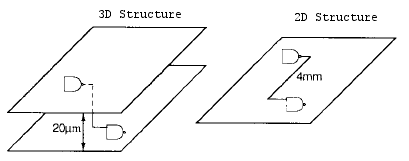
\includegraphics[width=0.75\linewidth]{wire.png}
\end{center}
\vspace{-0.5cm}
\caption{Shorter interconnections \cite{659500}}
\label{fig:wire}
\end{figure}

\paragraph{Silicon efficiency and accessibility}

Adding a vertical dimension allows to increase the integration density. It is therefore possible to have more logic gates than a 2D-IC for the same footprint, hence a more efficient use of the silicon as shown in Fig. \ref{fig:footprint}. For instance, compared to the footprint of a 2D-IC, the 3D-SICs can double the integration for a 50\% use of a 2D footprint \cite{659500}.

\begin{figure}[h!]
\begin{center}
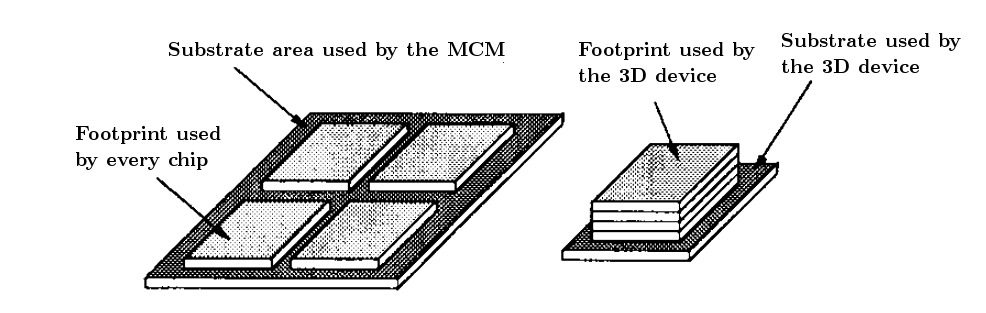
\includegraphics[width=0.75\linewidth]{footprint.png}
\end{center}
\vspace{-0.5cm}
\caption{Silicon efficiency \cite{659500}}
\label{fig:footprint}
\end{figure}

In addition, the 3D integration allows a better accessibility for the components, as shown in Fig. \ref{fig:accessibility}. Indeed, for a 2D structure, 8 accessible neighbours can be considered for a central element (Fig. \ref{fig:accessibility} (a)), whereas for a 3D structure, the number of accessible neighbours can reach 116 with through-tiers interconnections (Fig. \ref{fig:accessibility} (b)) \cite{659500}.

\begin{figure}[h!]
\begin{center}
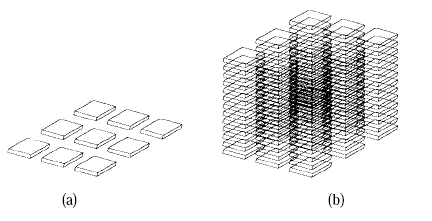
\includegraphics[width=0.75\linewidth]{accessibility.png}
\end{center}
\vspace{-0.5cm}
\caption{Components accessibility \cite{659500}}
\label{fig:accessibility}
\end{figure}

\paragraph{Bandwidth}

The use of TSVs on 3D-SIC can significantly increase the bandwidth of a circuit. Indeed, as shown in Fig. \ref{fig:bandwidth}, the interconnections are not only limited to peripheral connections but can also make use of the circuit's surface. This increase of the bandwidth allows higher working frequencies so that it is easier to satisfy data-heavy applications.

\begin{figure}[h!]
\begin{center}
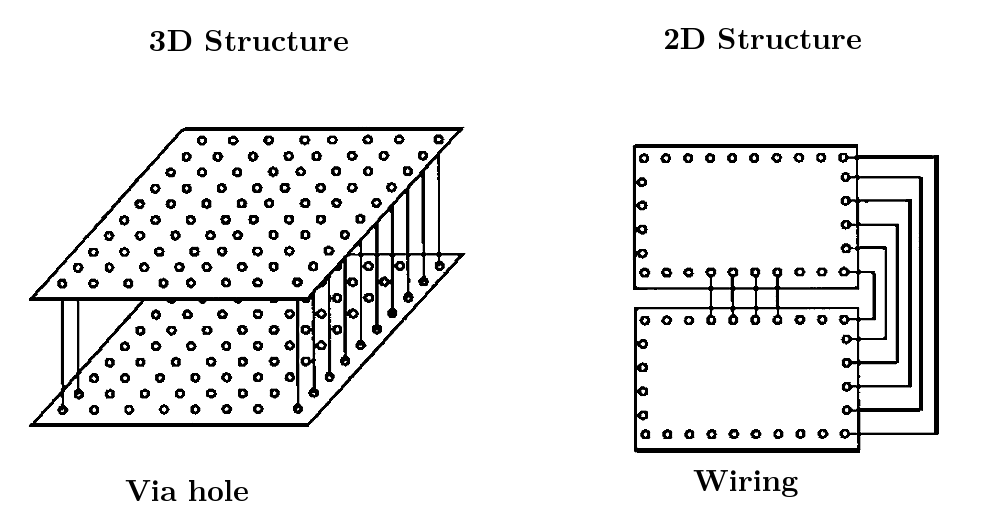
\includegraphics[width=0.75\linewidth]{bandwidth.png}
\end{center}
\vspace{-0.5cm}
\caption{Bandwidth improvement \cite{659500}}
\label{fig:bandwidth}
\end{figure}

\paragraph{Consumption and noise}

Shorter interconnections generally translates into lower capacitance and inductance parasites. This means a decrease of the numbers of repeaters, hence a better consumption, less noise and less jitter.

\paragraph{Heterogeneous circuits}

The 3D technologies allow truly heterogeneous designs. For instance, it is possible to integrate, in addition to traditional digital circuits of different technologies, analogical circuits such as sensors or antennas, as well as power supply, which give 3D-SIC a high degree diversity \cite{4299568}. The Fig. \ref{fig:heterogeneity} shows a schematic view of a 3D-SIC developed by IMEC for biomedical purposes that contains antennas, DSPs, EEG/ECG sensors, a power supply and solar cells \cite{4198870}.

\begin{figure}[h!]
\begin{center}
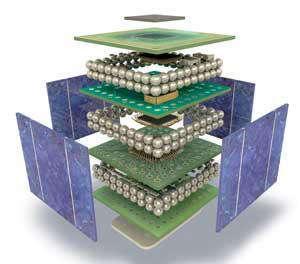
\includegraphics[width=0.5\linewidth]{heterogeneity.png}
\end{center}
\vspace{-0.5cm}
\caption{Schematic illustration of an heterogeneous 3D-SIC (developed by IMEC) \cite{4198870}}
\label{fig:heterogeneity}
\end{figure}

\subsection{Manufacturing technologies}

Several 3D manufacturing technologies have been proposed and have been used to implement complete systems. Among the existing possibilities, four major categories of methods that illustrate 3D integration can be cited \cite{659500,1652906}.

\paragraph{Chip stacking}

This methods consists in stacking components that have been designed and tested separately to produce a system-in-package (SiP). The vertically-stacked chips are interconnected with traditional wirings. The principal advantage of this method is an improvement in terms of size. The wirings are shorter however the components integration density is not increased compared to a 2D system.

\paragraph{Transistor stacking}

The transistor stacking consists in creating several transistors level on one substrate. This should be the better way to manufacture 3D circuits although the success rate are currently limited due to thermal issues. The required temperatures to create a layer of high-performance transistors would provoke the destruction of the copper and aluminium already laid down on the previous layer.

\paragraph{Die-on-wafer stacking}

In this method, known good dies (KGD), which are functional tested chips, are connected to a host wafer containing other KGDs. These KGDs can be interconnected with organic glues, oxide or metal bonding. The wafer and the bonded KGDs are then shaped to create the interconnections. Different substrates can be combined if the required temperature is low enough to minimize non-homogeneous expansion effects.

The die-on-wafer stacking can use interconnections on the edges of the chips or through-die. Depending on the interconnection type, this method can produce a better integration level than the chip stacking, with a better cost per connection ratio and a higher interconnection density, while holding the advantages of the KGDs.

The quality of the stacking depends on the pick-and-place equipment which is used to position the dies on the wafer. The placement accuracy will determine the possible interconnection density. Also, current equipments are supposed to handle fully buffered chips, not naked circuits so it does not provide protection to static discharge. 

\paragraph{Wafer-level stacking}

This methods consists in bonding entire wafers into a stack. The vertical through-wafer connections are made directly trough each substrate to the next wafer and it transistors layer. Similarly to the previous method, the interconnection density rely on the precision of the alignment, which is however currently better than the die-on-wafer stacking. This greater accuracy implies a better cost per connection ratio and a higher interconnection density compared to the die-on-wafer stacking.

The use of mixed substrates is also possible, only limited by the process temperatures. All the processing is done at the wafer level so wafer handling equipments are used. Since these provide protection to static discharge so there is no need to include buffering between the layers. The methods to bind two wafers are the same that are available for the die-on-wafer method.

One drawback to wafer-level stacking is its efficiency, since the chips on a wafer are not all KGDs.

\subsection{3D-SIC design challenges}

As explained, 3D-SICs offer numerous design perspectives thanks to their advantages. However there are drawbacks that need to be taken into account and that will be discussed in the following paragraphs.

\paragraph{Thermal dissipation}
The power density has increased exponentially over the past decades for the 2D-ICs and it appears that this trend will continue in the near future. As for 3D-SICs, due to their higher component density, they will also be subject to higher power density so thermal management should be considered carefully \cite{659500}. A simplified model of thermal dissipation has been developed in this thesis and will presented in Chapter \ref{cha:model}.

\paragraph{Cost}
With the appearance of a new technology, the involvement of a high cost should often be expected. In the case of 3D technology, the cost is currently high due to the lack of infrastructure and the reluctance of manufacturers who do not want to risk to change to new technologies \cite{659500}.

\paragraph{Design complexity and design software}
A large number of systems have been implemented using the 2D technologies which means that current tools can cope with 2D design complexity even if they show more and more their limits \cite{vanderbiest06, PFF10}. As for 3D-SICs, the increased complexity can be tackled by developing adapted software \cite{659500}. However, to the best of our knowledge, few 3D dedicated software currently exist and they are mainly developed for and owned by particular manufacturers and are based on 2D design tools which does not allow to tackle the complexity of 3D designs integrally.

In the following section, we will have an overview about these software tools and generally about the design flow used to design integrated circuits;

\section{Current design flows and their limitations}

Design flows are the combination of electronic design automation (EDA) tools used to produce an integrated circuit. These flows can generally be summarized in 4 main steps \cite{coursefred}, as shown in Fig. \ref{fig:designflow}.

\begin{figure}[h!]
\begin{center}
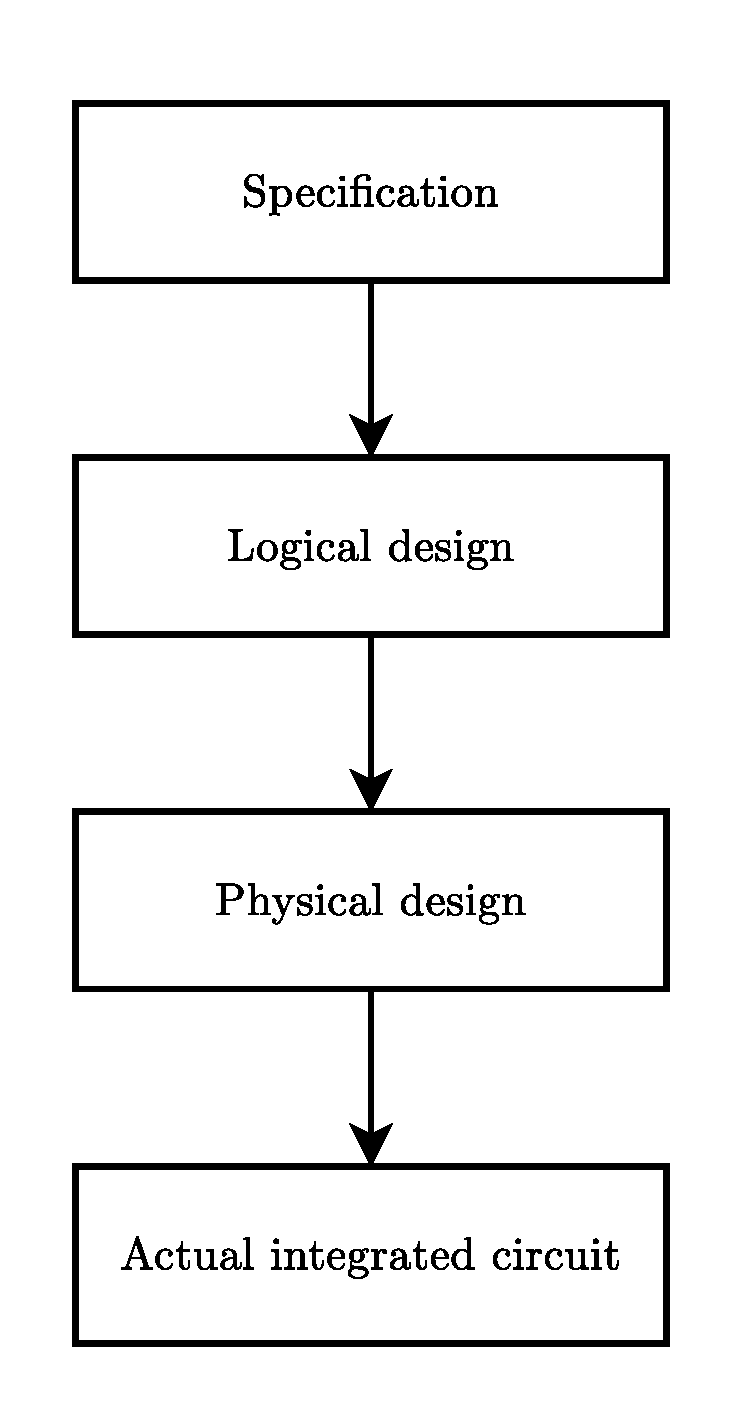
\includegraphics[width=0.35\linewidth]{designflow.eps}
\end{center}
\vspace{-0.5cm}
\caption{General classical design flow}
\label{fig:designflow}
\end{figure}

As explained previously, designing ICs implies numerous choices. At the moment, with this growing complexity, the current design flows can already show their limits. For instance, most of the time, the designers will be likely to freeze a certain amount of choices on basis of their experience, and then begin the optimization process with the remaining parameters. This will therefore limit the exploration of the design space and other good solutions may be ignored. In addition, the fixed choices can be questionable since they are based on the designer's experience though they could also be based on more objective facts.

The current design flows, which already showed their limits with conventional 2D-ICs, may thus need improvements to be able to deal with the increased complexity of emerging 3D-SICs \cite{vanderbiest06, PFF10}.

\section{Design space exploration tools}

In order to cope with the increasing complexity of integrated circuits and the limitations of the current design flows, numerous tools have been proposed, in particular works about design space exploration (DSE) that have been developed to quickly suggest possible interesting solutions to a designer and speed up the design processes. In this section, we will describe different DSE tools that have been proposed in the literature.

\subsection{2D-IC tools}

\paragraph{MILAN}

The MILAN (Model based Integrated simuLAtioN) framework \cite{Mohanty02rapidsystem-level} aims to simplify the optimization and the exploration of design spaces for SoC platforms. This tool works on the component level and allows the users to choose a compromise between the simulation speed and the results accuracy. The exploration and optimization process is done in two phases: first it searches for possible combinations between the architecture, the application and the mapping and second it estimates the performances (power, latency) depending the precision asked by the users.

\paragraph{SoC Architecture Explorer}

SoC Architecture Explorer \cite{ueda05architecture} is a multi-objective optimization and exploration tool that aims the design of SoC architectures by evaluating the compromises between the footprint and the execution time. The exploration process focuses on the application and the system architecture where the tool analyses the data flow and estimates the data transfers to determine a number of possible architectures.

%http://www.esteco.com/index.jsp
\paragraph{modeFRONTIER (ESTECO)}

modeFRONTIER \cite{esteco01} is a proprietary development environment developed by ESTECO. It is a multi-objective optimization tool that aims parallel SoC architectures. modeFRONTIER allows to deal with up to one million different design configurations thanks to statistical analysis tools and data mining techniques.

%http://www.multicube.eu/
\paragraph{MULTICUBE}

The MULTICUBE project (MULTI$^{3}$) \cite{multicube08, Silvanoetal09} is a European project started in 2008 and dedicated to the multi-objective exploration of MPSoC architectures for multimedia embedded systems. The aims is to developed a framework that allows a quick and automated exploration of the design space to improve the performances of a MPSoC with metrics such as power, latency, computing performance, bandwidth, QoS, etc. This project is based on several heuristics and optimization algorithms that reduce the exploration time and allow a quick selection of the best solutions of a Pareto-optimal frontier. In addition, MULTICUBE also aims to define an application-oriented framework based on the results of the multi-objective exploration to optimize the resources allocation and the tasks scheduling of the applications. The exploration is done at the system level, using the SystemC language. The project includes proprietary and open-source tools whose development targets the industry. Among the developed prototyping tools, Multicube explorer and Multicube-SCoPE can be cited.

%http://home.dei.polimi.it/zaccaria/multicube_explorer_v1/Home.html
\subparagraph{Explorer}

Multicube Explorer \cite{m3explorer09} is a design space exploration framework for supporting platform-based design. This tools allows a fast optimization of a system with objective functions such as power, delays, surface, etc. by means of a system simulator. Multicube explorer proposes several multi-objective optimization methods that aim to propose the best compromises.

%http://www.teisa.unican.es/gim/en/scope/multicube.html
\subparagraph{Multicube-SCoPE}

Multicube-SCoPE \cite{m3scope09} is an evolution of the SCoPE tool \cite{scope04} oriented to design space exploration. It is a fast system performance and power simulator providing metrics associated with a system in order to drive the DSE process.

%\cite{,, , 4735042, }
\subsection{3D-SIC tools}

\paragraph{DSE for 3D-stacked DRAMs by Weis \textit{et al.}}
Design space exploration for 3D-stacked DRAMs has been developed by Weis \textit{et al.} \cite{5763068}. They defined a model for 3D-DRAM and evaluated the performance of different DRAM architectures and technologies. This allowed them to have a the trade-off analysis of horizontal wirings against vertical wirings in terms of energy and cell efficiency.

\paragraph{DSE for 3D architecture by Xie \textit{et al.}}
Design space exploration for 3D architecture is a work proposed by Xie \textit{et al.} \cite{Xie:2006:DSE:1148015.1148016}. They combined the use of an analysis tool for 3D cache design with an thermal-aware 3D floorplanner to perform the DSE. This allowed them to consider performance, power and thermal for a 3D design. 

\paragraph{DSE for 3D integrated circuits by Xie \textit{et al.}}
Design space exploration for 3D architecture is another work proposed by Xie \textit{et al.} \cite{4735042}. They based this research on their previous one and extended it to add cost analysis.

\paragraph{Automated design flow for 3D microarchitecture evaluation by Cong \textit{et al.}}
An automated design flow for 3D microarchitecture evaluation has been proposed by Cong \textit{et al.} \cite{1594713}. They proposed an evaluation flow for performance assessment and thermal management. This allowed them to perform thermal-aware 3D floorplanning.

\paragraph{PathFinding flow}
The PathFinding flow is a project led by IMEC and Milojevic \textit{et al.} \cite{5335663,DBLP:conf/3dic/MilojevicCCRRSAPM09}. The aim of this work is to be able to produce a specification for the architecture and for the technology with assessment of performance, power and cost. The methodology is divided in 3 steps:
\begin{enumerate}
\item 3D system level design exploration with a rough estimation of the performance, power and cost parameters. The designer will be able to focus on the 2D design issues while manually considering the 3D specificities.
\item RTL (Register Transfer Level) elaboration, which links the system level to the physical design by producing RTL models.
\item 3D physical design prototyping, which allows fast exploration of the physical design impact of alternative design/technology options on the performance, power and cost parameters.
\end{enumerate} 

\section{Conclusion}
To the best of our knowledge, all these tools use a uni-criterion approach or deal with a limited set of criteria while performing only trade-off analyses from a Pareto front. The goal of this research is to show that a more multicriteria-oriented optimization could be more suitable to take into account the many aspects of a design and provide more information.

In the next chapter, we will describe a short overview of the tools coming from the operations research that will allow to take into account multiple criteria simultaneously.